\chapter{Conceitos Utilizados}

\section{Tecnologia de comunicação}
A partir de todo o levantamento teórico e considerando-se o contexto do problema, a tecnologia que mostrou mais destaque, foi o Bluetooth.

Mais especificamente, a introdução do Bluetooth Low Energy (BLE) tornou tal tecnologia bem favorável ao uso para localização, devido ao seu baixo consumo energético, mantendo caracteristicas similares de comunicação.

As principais características da escolha podem ser encontradas abaixo:

\begin{itemize}

    \item \textbf{Economia e eficiência energética}

    Uma das principais vantagens da tecnologia Bluetooth para a localização indoor é sua alta eficiência energética. O custo da instalação de um sistema com BLE é baixo quando em comparação de outras tecnologias já que um dispositivo equipado com um chip de BLE pode de 1 a 2 anos com uma unica bateria moeda (\textit{coin cell}).No contexto de um armazém, a economia de custos é fundamental.

    \item \textbf{Acessibilidade e Escalabilidade}

    Como mencionado, estima-se que até 2022 400 milhões de dispositivos de localização baseados em Bluetooth sejam vendidos por ano \cite{art9}. Fazendo-o uma tecnologia prontamente acessível e com vários recursos de desenvolvimento.

    Para o contexto do projeto, uma rápida implementação é desejável. Além disso, estar presente em dispositivos atuais é um requisito, dado que se deseja a instalação do sistema com o minimo de mudança na infraestrutura atual. Bluetooth está presente na maioria dos telefones celulares, os quais poderiam se integrar ao sistema prontamente.

    \item \textbf{Precisão}

    A precisão necessária é tal que dois SKUs (Unidade de Manutenção de Estoque) em localidades diferentes possam ser diferenciados. Para isso, uma precisão de até 1m é desejada.

    Com a tecnologia Bluetooth e os algoritmos corretos tal precisão pode ser alcançada.

    \item \textbf{Latência}

    A latência no Bluetooth é elevada quando comparada à outras tecnologias. Para aplicações que precisão de localização em tempo real pode ser uma desvantagem. Entretanto no projeto em questão os ativos ficam estáticos no armazém. E a latência não se torna um problema tão grande.

\end{itemize}

Antes de entrar no nas especificidade das propriedades do sinal utilizadas, cabe aqui um detalhamento do protocolo de Bluetooth Low Energy (BLE).

\subsection{Protocolo Bluetooth Low Energy}

O Bluetooth Low Energy (BLE) foi introduzido na especificação 4.0 do padrão IEEE 802.15.1 pelo Bluetooth Special Interest Group (Bluetooth SIG). É classificado como uma rede de acesso pessoal sem fio (WPAN) de baixo consumo, latência e custo \cite{Bluetooth_SIG_Site}.
A arquitetura do stack do protocolo Bluetooth pode ser dividido em várias camadas conforme a imagem \ref{fig:ble-protocol-stack.png}. Cada camada tem uma função específica. Para o trabalho as partes mais relevantes do funcionamento do protocólo são as partes da Camada Física (PHY), Camada de Enlace (LL) e do Generic Access Profile (GAP).

\begin{figure}[H]
    \centering
    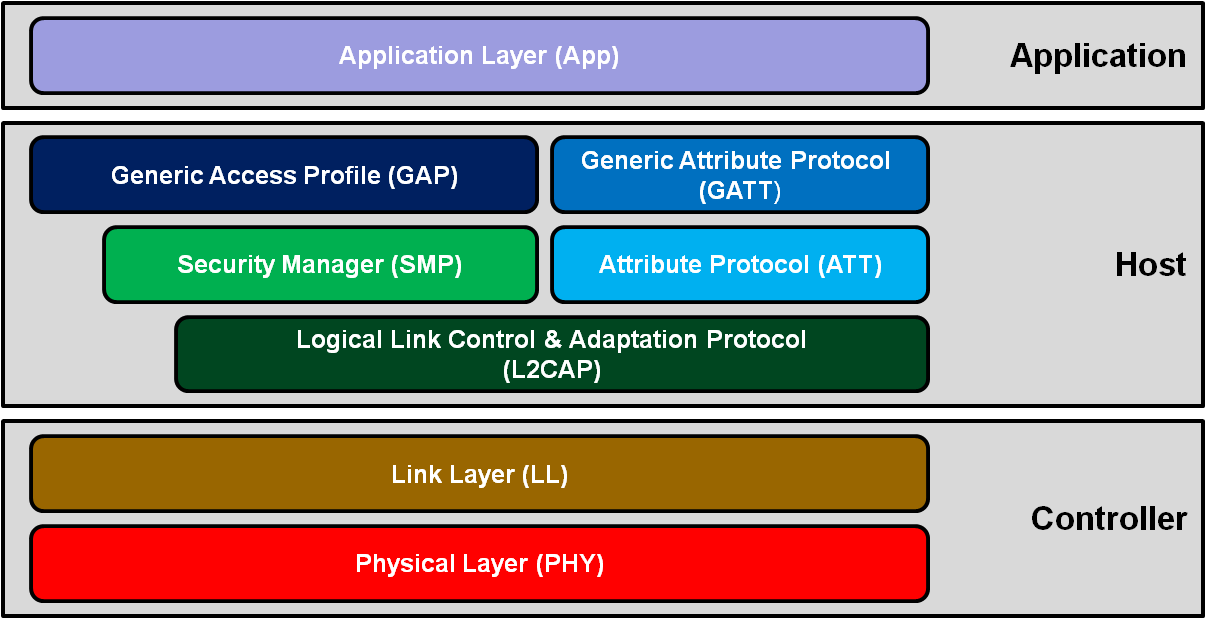
\includegraphics[width=1.0\textwidth]{images/ble-protocol-stack.png}
    \caption{Arquitetura do stack do protocolo Bluetooth. Tirado de \cite{Microchip_Site} }
    \label{fig:ble-protocol-stack.png}
\end{figure}



\begin{itemize}

    \item \textbf{Generic Access Profile (GAP)}
    
    As formas de operação do BLE são definidas pelo General Access Profile (GAP) e este perfil determina que um dispositivo possui 4 formas de operação:
    Broadcaster, Observer, Slave e Central.

    Como Broadcaster, o dispositivo opera somente como transmissor de dados, enviando pacotes de dados periodicamente, a cada ação denominada Advertising, que podem conter informações sobre o dispositivo e indicam a presença de um dispositivo num dado local. Quando um dispositivo opera apenas como broadcaster, ele não está aberto a receber conexões.

    Como Observer, o dispositivo opera somente como um receptor de dados, recebendo apenas os pacotes de advertising enviados por outros dispositivos BLE.
    
    Como Peripheral, o dispositivo suporta estabelecer uma conexão como escravo (slave). Para outro dispositivo detectar sua presença e iniciar uma conexão, é necessário que o peripheral opere antes como um broadcaster, indicando sua presença.

    Como Central, o dispositivo suporta múltiplas conexões como mestre (master) e é sempre o responsável por iniciar as conexões com um peripheral. Para detectar um peripheral, é necessário que a central opere como um observer para detectar a presença de outros dispositivos.

    Um dispositivo é capaz de suportar múltiplas formas de operação ao mesmo tempo \cite{Bluetooth_SIG_Site}.

    \item \textbf{Camada Física (Physical Layer - PHY)}
    
    A camada física contém o circuito analógico responsável pela transmissão de simbolos digitais pelo ar. É a camada mais baixa do stack e provém seus serviços para a camada de enlace (link layer). 

    Nessa camada, o BLE opera na banda 2.4GHz ISM (Industrial, Scientific, and Medical),contando com 40 canais de radio-frequências espaçados com 2Mhz entre si. Existem dois tipos de transmissão: a transmissão de dados, que é feita em 37 dos canais disponíveis com a capacidade de transmissão de 1Mbits, realizada pelos dispositivos operando como central ou com peripeheral; e o advertising, que é feito nos outros 3 canais restantes com as frequências de 2402MHz, 2426MHz e 2480MHz, que é realizado nos dispositivos operando como broadcaster. Esses são os canais 37, 38 e 39.

    Esses canais foram escolhidos propositalmente para diminuir a interferência com outros sinais da banda ISM, tais como os de Wi-fi (IEEE 802.11).

    \begin{figure}[H]
        \centering
        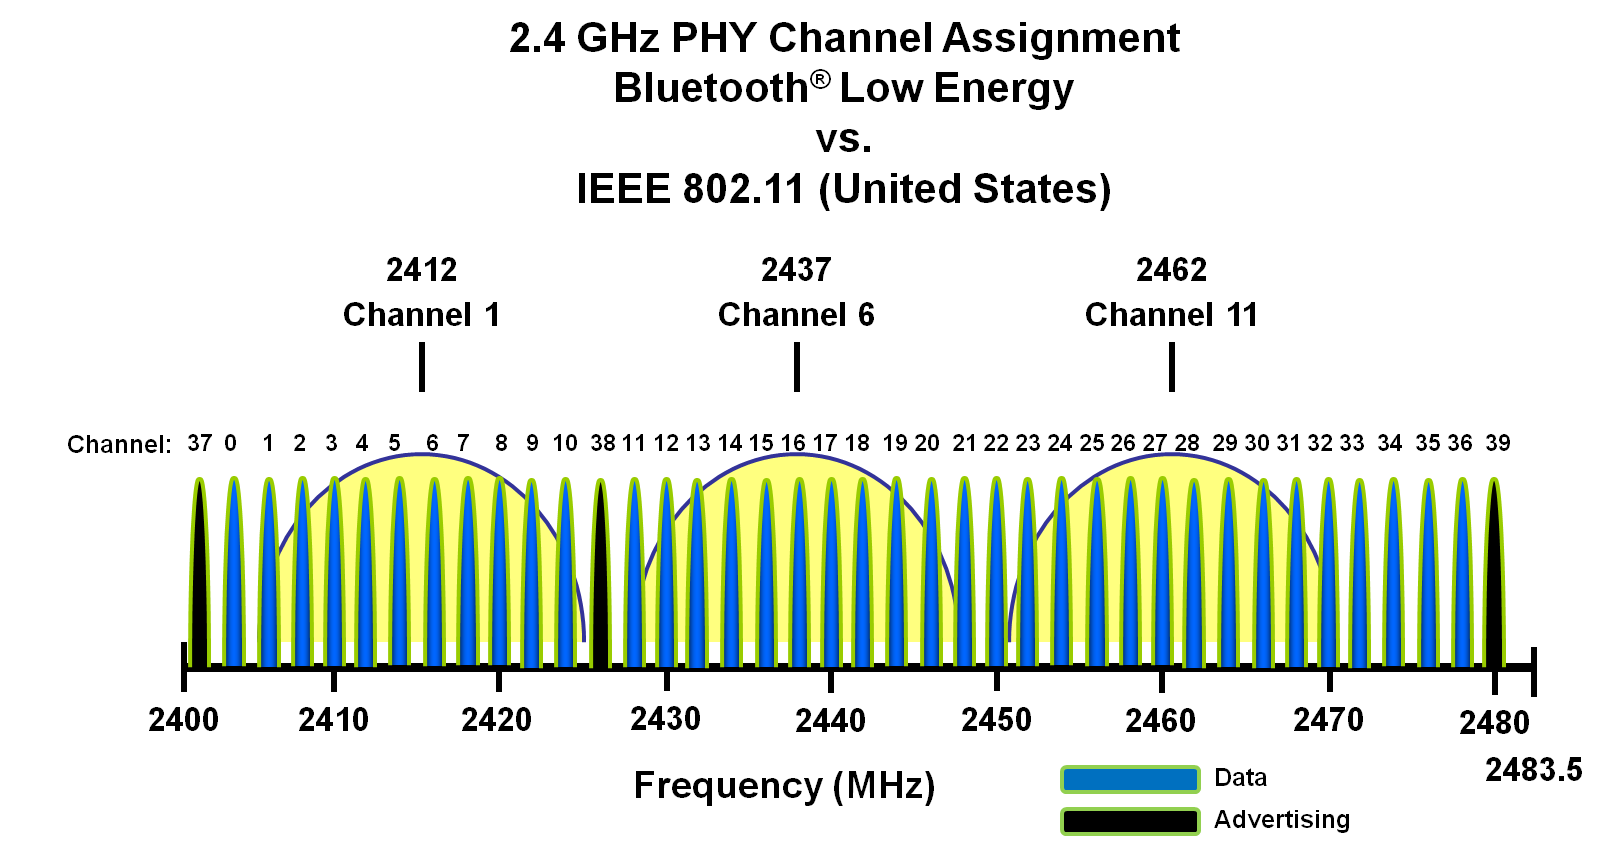
\includegraphics[width=1.0\textwidth]{images/ble-phy-channel-overlap.png}
        \caption{Canais do Bluetooth e de Wi-Fi. nota-se que os canais de advertising do BLE ficam em pontos que minimizam a interferência com os de WiFi. Tirado de \cite{Microchip_Site} }
        \label{fig:ble-phy-channel-overlap.png}
    \end{figure}
    
    
    Enquanto o modo de advertising utiliza os canais com menos interferencia da banda ISM, no modo conectado, o algoritmo FHSS (\textit{Frequency-hopping spread spectrum})é utilizado para diminuir interferências.

    É um algoritmo simples e pseudo-aleatório que dita qual vai ser o próximo canal que o BLE fará a transmissão de dados. Esse canal é alternado entre os 37 possíveis canais o que faz um distribuição de dados sobre eles mais igualitaria diminuindo interferências. Tanto o dispositivo oprando como peripheral quanto o central possuem acesso a esse algoritmo, sabendo qual vai ser o próximo canal em que se dará a comunicação.

    O próximo canal é dado pela seguinte formula:

    \begin{equation}
        f_{n+1} = (f_{n} + hop) mod 37
    \end{equation}

    Em que \( f_{n} \) é o canal atual da comunicação, \( f_{n + 1} \) é o próximo e \( hop \) é um valor que pode mudar entre 5 e 16 e é definido no momento em que uma conexão é estabelecida.

    O diagrama abaixo mostra que esse algoritmo provém um método robusto para manter uma conexão mesmo na presença de de interferências ou outros dispositivos de rádios no alcance do Bluetooth. No diagrama há 3 conexões de Bluetooth diferentes e o do 3 link está destacado para claridade.
    
    \begin{figure}[H]
        \centering
        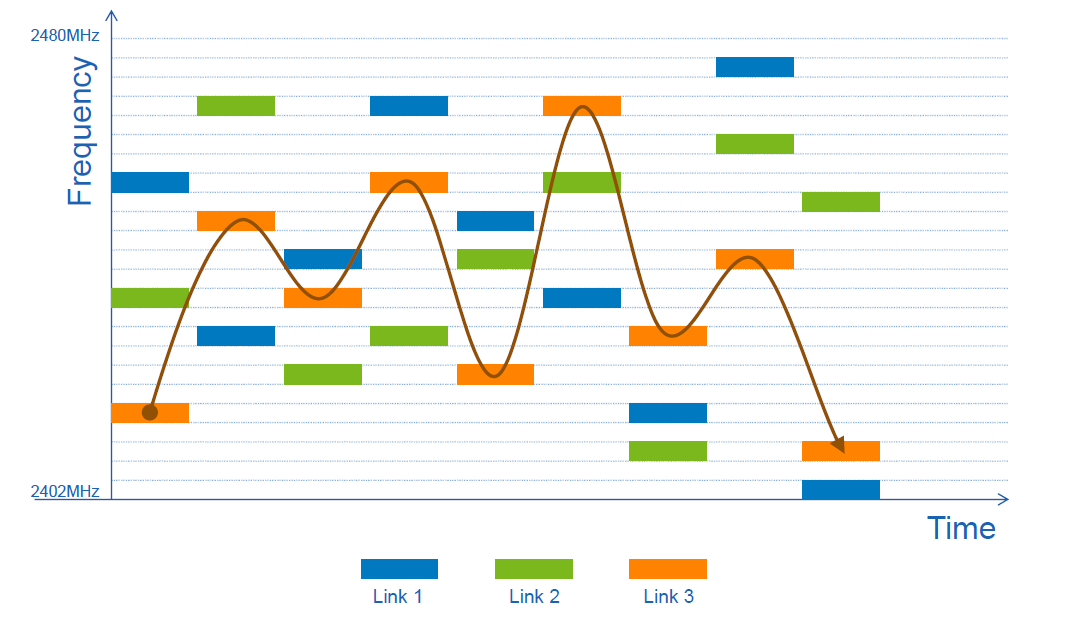
\includegraphics[width=1.0\textwidth]{images/frequency-hopping.png}
        \caption{\textit{Frequency Hopping Spread Spectrum} para 3 conexões. Tirado de \cite{Microchip_Site}}
        \label{fig:frequency-hopping.png}
    \end{figure}

    \item \textbf{Camada de Enlace (Link Layer - LL)}
    
    A Link Layer, é a responsável direta pela comunicação com a camada física. Ela é a responsável pelo advertising, o scanning, e criar e manter as conexões. Ele define quem inicia uma conexão, quando um dispositivo se conecta a outra ou quando fica em modo de stand-by. Os pacotes padrão de Bluetooth são especificados nessa camada.

    Os pacotes, chamados de PDU (Packet Data Unit) são constituidos de 2 bytes de cabeçalho seguidos de 255 bytes de payload no modo conectado e 37 bytes no modo de advertising. Para economizar energia o hardware entra em modo de sleep entre as transmissões. Além disso, um intervalo para transmissão de pacotes de advertising pode ser escolhido entre 20ms e 10.24 segundos. Quanto maior o intervalo, maior a economia de energia, porém menos possibilidade de uso em tempo real. 

  

\end{itemize}

\section{Propriedades do sinal}
Os principais algoritmos mencionados anteriormente exigem para sua implementação uma distância conhecida e um ângulo conhecido para um ponto de referência. No presente trabalho, será utilizado o RSSI como método principal para estimar a distância. %e o AoA para estimar o ângulo.

Quando um chip de Bluetooth recebe o sinal ele é capaz de retornar o valor da intensidade desse sinal, então a obtenção do RSSI é direta e não exige nenhum hardware adicional. Apesar de não ser o método mais preciso para estimar distância, seu custo benefício é alto.

Já para estimar o ângulo, o angle of arrival de um sinal poderia ser utilizado. Tal propriedade em conjunto com a de intensidade do sinal permite que algoritmos estimem uma localização com uma precisão maior quando em comparação a algoritmos que utilizam apenas a intensidade do sinal. Assim, apesar de necessitar de um hardware mais complexo, há um ganho significativo.

\subsection{RSSI}
O RSSI, como uma propriedade bruta do sinal adquirida pelo stack de Bluetooth, fornece uma precisão de menos de 10m. Valor relativamente alto para a realização de localização indoor. Entretanto, é possível melhor essa precisão com algumas técnicas, em hardware, firmware e software.

Na aquisição do sinal, foi implementado uma técnica para a obtenção da intensidade do sinal em cada um dos três canais de advertising (canal 37, canal 38 e canal 39) separadamente, em contraste com a abordagem clássica de obter o RSSI de todos os canais de advertising simultaneamente, o que permite uma maior precisão no uso do RSSI. A dificuldade desse método aparece porque o padrão BLE nativo, não provém uma API para recuperar informação dos canais de advertising na recepção dos pacotes transmitidos, assim pequenos ajustes no stack de bluetooth devem ser feitos \cite{art16}.

Essa técnica melhora a precisão do RSSI em relação com a obtenção de todos os sinais simultaneamente pois assim é possível fazer uma análise personalizada para cada um dos canais, mitigando efeitos de interferências entre os canais, efeitos de \textit {fading} e eventuais erros na transmissão de dados \cite{art17}.

Uma vez coletada a informação dos canais separadamente, deve-se tratá-los adequadamente. Dependendo da situação, uma das formas de tratamento a seguir foi utilizadas :

\begin{itemize}

    \item Utililzar dados somente do canal que está fornecendo o maior valor de RSSI. O canal que é considerado como dando a maior precisão é o que fornece maior RSSI nesse caso:

    \begin{equation}
        RSSI_{max} = max(RSSI_{ch37}, RSSI_{ch38}, RSSI_{ch39})
    \end{equation}

    \item  Utilizar a média dos calores obtidos em todos os canais. Usando a média dos três canais, eventuais erros em um canal tem seu efeito minimizado:

    \begin{equation}
        RSSI_{average} = \frac{1}{3} \sum_{i=37}^{39}  RSSI_{ch i}
    \end{equation}


    \item Obter o valor do RSSI pela combinação de razão máxima (\textit{Maximum Ratio Combining} - MRC). Essa abordagem coloca peso nos canais de forma que a combinação resultante dê uma enfasê maior para os canais com maior leitura de RSSI do que para os canais com menor leitura, porém os com menor leitura ainda são levados em conta:

    \begin{equation}
        RSSI_{MRC} = \sum_{j=37}^{39} \frac{RSSI_{ch j} - RSSI_{min}}{\sum_{i=37}^{39}  RSSI_{ch i}} RSSI_{ch j}
    \end{equation}

    Em que o valor de \( RSSI_{min} \) foi escolhido de acordo com a mínima sensibilidade do módulo bluetooth utilizado.


\end{itemize}

A partir do valor de RSSI que foi estimado com base no RSSI dos três canais, utilizou-se a triangulação para a determinação da posição de acordo com as equações de \ref{sec:trilateracao}.

Nas imagens \ref{fig:rssi_channels_raw.png} e \ref{fig:rssi_channels_mrc.png} tiradas de \cite{art17}, é possível perceber a diferença que a leitura separada dos canais pode fazer. Na imagem \ref{fig:rssi_channels_raw.png}, tem-se a leitura bruta dos valores dos canais para 500 medições, nessa caso há uma alta dispersão dos dados para um mesma distância, demonstrando a necessidade de algum tipo de tratamento dos dados.
Na imagem \ref{fig:rssi_channels_mrc.png}, utilizou-se o método do MRC descrito acima. Neste caso, há uma flutuação bem menor dos dados, o que é crítico para uma localização precisa.

\begin{figure}[H]
    \centering
    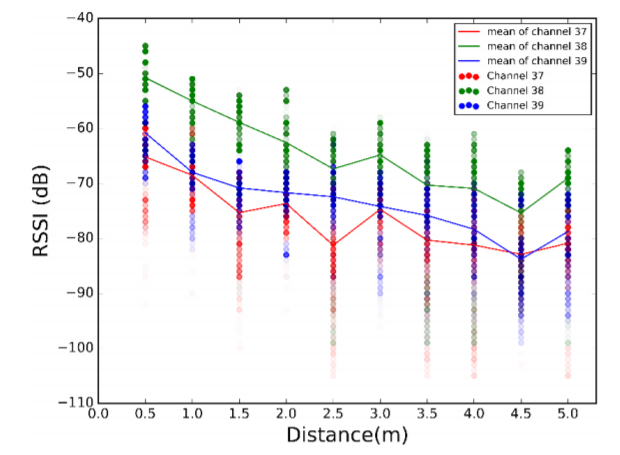
\includegraphics[scale = 1]{images/rssi_channels_raw.png}
    \caption{Gráfico de dispersão do RSSI medido para diferentes distâncias conhecidas para diferentes canais sem tratamento.  \cite{art17}}
    \label{fig:rssi_channels_raw.png}
\end{figure}

\begin{figure}[H]
    \centering
    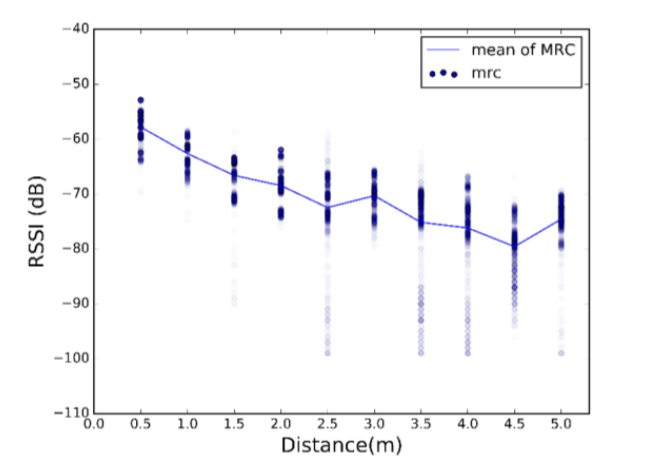
\includegraphics[scale = 1]{images/rssi_channels_mrc.png}
    \caption{Gráfico de dispersão da média do RSSI calculado por meio do algoritmo MRC \cite{art17}}
    \label{fig:rssi_channels_mrc.png}
\end{figure}



\subsection{Angle of Arrival}
O Angle of Arrival (Ângulo de Chegada), foi detalhado em \ref{sec:AoA}, e é uma propriedade capaz de incrementar bastante a precisão da localização indoor. Alguns estudos alegam que é possível obter precisão de centímetros usando essa propriedade do sinal com os algoritmos adequados \cite{art9}. O problema dessa abordagem entra na grande dificuldade da realização desses algoritmos que permitam uma estimativa precisa de ângulo. 

Para o trabalho, a abordagem de AoA não foi implementada, dado que o RSSI separado por canais forneceu uma precisão aceitável para a localização e a abordagem profunda da implementação algoritmos para estimar bem o AoA acabaria fugindo do escopo do projeto, entretanto, dada sua tamanha importância na melhoria de precisão e nos futuros trabalhos de localização indoor, será dado uma explicação da teoria por trás da obtensão do angulo de chegada do sinal de bluetooth e como esse ângulo pode fornecer a posição do que se deseja localizar.


Em primeiro lugar, para se obter a direção de um sinal é necessário um array de antenas, responsável por extrair a informação de ângulo do sinal recebido. 

Esse array de antenas pode estar ou no dispositivo a ser localizado ou no localizador. No caso de o dispositivo a ser localizado possuir um array de antenas para estimar o ângulo de chegada o termo utilizado é AoA (Angle of arrival), já no outro caso o processo é chamado de AoD (Angle of Departure). Os dois casos utilizam os mesmos princípios e podem ser mais ou menos convenientes em cassos específicos. \cite{techreport1}
Aqui será referido o AoA, porém a teoria é a mesma para o AoD.

Para longas distancias a onda de rádio transmitida pode ser vista como uma onda planar ao invés de esférica. Se essa onda se propagar na direção normal do array de antenas do receptor cada uma das antenas do array vai receber a mesma fase da onda. Entretanto, quando se quer obter o angulo de um sinal, evita-se deixar nessa posição, de talforma que cada antena do array de antenas recebe a onda com uma fase diferente. Essa informação de diferença de fase faz com que seja possível estimar o nâgulo de chegada de um sinal.

Na literatura essas amostras de diferentes fases do sinal pelo array de antenas são chamados de "IQ-Samples" (In-phase and Quadratura-phase samples). Para a maioria dos algoritmos de estimativa de ângulo por meio dos IQ-Samples é necessário uma defasagem máxima de 90 graus entre as amostras. Considerando-se a velocidade da luz como \( 300.000 km/s \) e a frequência do sinal do bluetooth aproximadamente \( 2.4 GHz \) para uma defasagem de 90 graus é necessario um espaçamento L máximo de \( L = (3 * 10^8)/(2.4 * 10^9) = 0.125m \). Já o espaçamento mínimo é limitado pela tecnologia e não há um limite teórico.

Os desafios técnicos para a obtenção do ângulo por meio do array de antena se deve ao fato de que os ambientes onde se realizará a amostragem não são ideais. O que faz com que haja sinais "multi-path" que são basicamente uma versão atrasada do mesmo sinal, por reflexões on ambiente, por exemplo. Ou ainda ruídos no ambiente que não podem ser isolados. Por último tem-se o problema que no geral os sistemas embarcados que fazem a coleta dos IQ-Samples, não tem memória limitada, o que dificulta a realização de algoritmos completos no proprio dispositivo.

Para a superação desses desafios, algoritmos rubustos tiveram que ser desenvolvidos para estimar o ângulo do sinal com base nas amostras. Aqui serão apresentados dois deles em nível alto sem provas do motivo pelos quais funcionam: o Classical Beamformer e o MUSIC:

\begin{itemize}

    \item \textbf{Classical Beamformer}
    
    Considerando-se um vetor de IQ-Samples para cada antena dado por \( x \), pode-se modelar esse vetor pela seuinte equação:

    \begin{equation} \label{eq:eq_iq}
        x(t) = a(\theta)s(t) + n(t)
    \end{equation}

    Em que  \( n(t) \) é um modelo de ruídos, \( s(t) \) é o sinal que foi transmitido no ar e \( a \) é o vetor de posição do array de antenas, dado por:

    \begin{equation} \label{eq:eq_steering_vector}
        a(\theta) = [1, e^{j2\pi d sin(\theta)/\lambda}, ... , e^{j2\pi (m-1) d sin(\theta)/\lambda}]
    \end{equation}

    Em que \( d \) é a distância entre as antenas, \( \lambda \) o comprimento de onda do sinal transmitido, \( m \) o número de elementos no array de antenas e \( \theta \) o ângulo de chegada

    O vetor de posição \ref{eq:eq_steering_vector} descreve como os sinais em cada antena são deslocados de fase devido às diferentes distâncias para o transmissor. Usando \ref{eq:eq_iq}, podemos calcular uma aproximação da chamada matriz de covariância da amostra, \( R_{xx} \), essa matrix auxilia depois para encontrar o ângulo:

    \begin{equation} \label{eq:eq_Beamformer}
        R_{xx} = \frac{1}{N}\sum_{t=1}^{N}x(t)x^{H}(t)
    \end{equation}

    Em que H é a transposição hermitiana de uma matriz.

    Finalmente, a parte central do algoritmo, se dá ao se achar \( \theta \)  que máximiza a potencia \( P(\theta) \) na seguinte equação:

    \begin{equation} \label{eq:eq_rxx}
        P(\theta) = \frac{a^{H}(\theta)R_{xx}a(\theta)}{a^{H}(\theta)a(\theta)}
    \end{equation}

    Esse \( \theta \) encontrado é a melhor estimativa para o ângulo de chegada nesse algoritmo. Porém ainda assim não é muito preciso, e robusto, apesar de uma simplicidade maior em relação ao próximo.

    \item \textbf{MUSIC (Multiple Signal Classification)}
    
    A ideia desse algoritmo é realizar uma decomposição dos autovalores e autovetores da matriz \( R_{xx} \):

    \begin{equation} \label{eq:eq_autovalores_rxx}
        R_{xx} = VAV^{-1}
    \end{equation}

    A partir disso é possível construir um pseudo-espectro P para o sinal dado por:

    \begin{equation} \label{eq:eq_music}
        P(\theta) = \frac{1}{a^{H}(\theta)VV^{H}a(\theta)}
    \end{equation}

    E realizando-se um procedimento similar ao algoritmo de cima, encontrando-se o \( \theta \) que máximiza a equacão \ref{eq:eq_music}, encontra-se o ângulo de chegada mais provável. Esse é um algoritmo bem robusto que fornece boas precições. Entretanto seu peso computacional é alto.


\end{itemize}

As referências \cite{art19}, \cite{techreport1} e \cite{art20} dão mais detalhes dos algoritmos mencionados e realizam experimentos demonstrando seus usos.


%Vale ressaltar o ble 5.1
% \todo{5.1}

Nas especificações do Bluetooth anteriores à 5.1 lançada em janeiro de 2019, a obtenção do AoA exigia um hardware extra.
Entretanto, dados os recentes avanços na tecnologia agora é possivel estimar o ângulo de chegada de um sinal se o chip Bluetooth utilizado possuir suporte para Bluetooth 5.1 ou superior.

Uma alternativa para estimar o AoA para especificações anteriores à 5.1 é a utilização de um interferômetro de 6-portas, que é um dispositivo que é baseado nas superposições deslocadas de fase das ondas incidentes e refletidas em uma porta. Diferentes defasagens de fase resultam em diferentes potências nas portas de saída da arquitetura de um 6-portas \cite{art14}.

Abaixo um desenho esquemático da arquitetura de um 6-portas:

\begin{figure}[H]
	\centering
	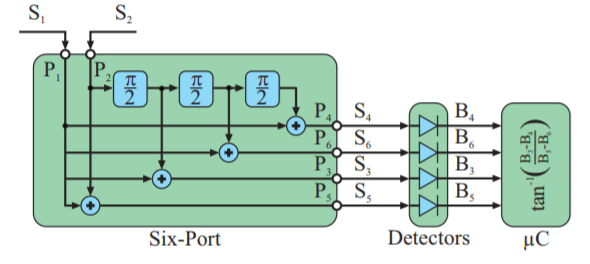
\includegraphics[scale = 1]{images/six_port_schematic.png}
	\caption{Esquemático de uma arquitetura 6-portas. Tirado de \cite{art15} }
	\label{fig:six_port_schematic}
\end{figure}

Na figura \ref{fig:six_port_schematic} os símbolos \( S_1 \) e \( S_2 \) representam os de sinais de entrada e \( S_3 \) a \( S_6 \) representam as potências medidas na saída. Já os simbolos de \( B_3 \) a \( B_6 \) representam as potências de \( S_3 \) a \( S_6 \) convertidas para tensões de base.

As equações que relacionam esses sinais são:

\begin{align*}
    S_3 & = 0.5(S_1 + jS_2) & B_3 = \left | S_3 \right | ^2\\
    S_4 & = 0.5(S_1 - jS_2) & B_4 = \left | S_4 \right | ^2\\
    S_5 & = 0.5(S_1 + S_2)  & B_5 = \left | S_5 \right | ^2\\
    S_6 & = 0.5(S_1 - S_2)  & B_6 = \left | S_6 \right | ^2
\end{align*}

A partir disso, é possível encontrar diversas propriedades úteis dos sinais incidente, tais como a a diferença de fase \( \Delta\phi\), a distância do sinal \( \Delta\delta\) e a propriedade do ângulo de chegada \(\theta\) a partir das seguintes equações:

\begin{equation}
    Z = (B_5 - B_6) + j(B_3 - B_4)
\end{equation}

\begin{equation}
    \Delta \phi = \arctan \left ( \frac{B_3-B_4}{B_5-B_6} \right )
\end{equation}

\begin{equation}
    \Delta d = \lambda \frac{\arg\left ({Z}  \right ) }{4\pi }
\end{equation}

\begin{equation} \label{eq:eq_AoA}
    \theta = \sin^{-1}{(\frac{\lambda \Delta \phi}{2\pi a} )}
\end{equation}

Em que Z é um número complexo que relaciona as tensões de saída, \(\lambda\) é o comprimento de onda do sinal e \(a\) a distância entre antenas receptoras.

A referência \cite{art15} apresenta um maior detalhamento da arquitetura. Para o contexto de localização indoor, as equações forneceriam o ângulo \(\theta\) desejado.

\section{Algoritmos}

% \todo{Algoritmos}

\section{Camada de Aplicação}

% \todo{Teoria Aplicacao}
